%% Mans Maģistrs
\documentclass[magjistrs]{vea-diplomdarbs}
\usepackage{setspace}	% Line spacing package
\usepackage{calc}
\usepackage{booktabs}
\usepackage{tabularx}
\usepackage{amsmath}

\usepackage[title,toc]{appendix}
\renewcommand{\setthesubsection}{\Alph{subsection}}

%% Use proper Aurora Bold Condensed BT
\definecolor{SeaBlue}{cmyk}{1,0,0.37,0.52}
\newfontfamily\TitleFont[%
	Path = /home/johnlm/Development/resources/tex_graphics_lib/fonts/ ,%
	FakeStretch = 1.5 ,
	Color = SeaBlue
	]{aurora-BT-condensed-bold}

\setotherlanguages{english,russian}

% Russian Font
\newfontfamily\cyrillicfont{CMU Serif}	% Unicode Computer modern font

\newcommand{\TODO}{\textcolor{red}{TODO}}

%% Inline Word inclusion formatting
\newcommand{\termEn}[1]{\textenglish{\itshape {#1}}} % inline English
\newcommand{\termLatin}[1]{\textit{#1}} % inline Latin
\newcommand{\termTech}[1]{\textit{#1}} % technical term (LV?)
\newcommand{\newTerm}[1]{,,{#1}''} %newly mentioned term

%% Pāris matemātikas komandu definīcijas
\newcommand{\vb}[1]{\mathbf{#1}}
\newcommand{\units}[1]{\;\mathrm{#1}}

%% English determined number suffixes
\newcommand{\st}{\textsuperscript{st} }
\newcommand{\nd}{\textsuperscript{nd} }
\newcommand{\rd}{\textsuperscript{rd} }
\newcommand{\nth}{\textsuperscript{th} }

%% Abstract title style
\newcommand{\abstitlestyle}[1]{%
	\noindent \begin{center}
		\textbf{\Large #1}
	\end{center}}


\hyphenpenalty=7500
\clubpenalty=9000
\widowpenalty=9000

\title{Attēlu raksturpunktu pāru noteikšanas algoritmu ātrdarbības izpēte dažādām aparatūras platformām}
\author{Jānis Šmēdiņš}

% Hyperref package for links in PDF (should be last package)
\usepackage[hyperfootnotes=false,linkbordercolor={blue},hyperindex]{hyperref}
\hypersetup{pdftitle={Attēlu raksturpunktu pāru noteikšanas algoritmu ātrdarbības izpēte dažādām aparatūras platformām}}
\hypersetup{pdfauthor={Jānis Šmēdiņš}}
\usepackage{fixlatvian}

\begin{document}
	% Titullapa
	\pagestyle{empty}
	% LM izcilā VeA titullapa bakalauram!
\begin{titlepage}
	% VeA Logo
	% "Ventspils Austskola" virsraksts (\TitleFont jābūt definētam!!!)
	\newsavebox{\veatext}
	\savebox{\veatext}{
		\TitleFont\Huge\MakeUppercase{Ventspils Augstskola}}
	% Teksta platuma noteikšana (lai pielīdzinātu bildi tā platumam}
	\newlength{\veatextwidth}
	\settowidth{\veatextwidth}{\usebox{\veatext}}
	% Šeit drukāts pats logo un nosaukums
	\centering\includegraphics[width=0.98\veatextwidth]{VeA_logo.pdf}\\[4pt]
	\usebox{\veatext}\\[6pt]
	\large Informācijas tehnoloģiju fakultāte\\[2cm]
	
	\textbf{Bakalaura darbs}\\[1.5cm]
	%\textbf{Bakalaura darba 1.~atskaite}\\[1.5cm]
	
	\textsc{\LARGE Iekļautās sistēmas mikrokontroliera kodola izstrāde}
	\vfill % LIELĀ atstarpe
	
	%\raggedleft
	\normalsize
	\begin{minipage}[t]{0.4\textwidth}
		\begin{flushleft}
			Autors
		\end{flushleft}
	\end{minipage}
	\begin{minipage}[t]{0.55\textwidth}
		\begin{flushleft}
			Ventspils Augstskolas \\
			Informācijas tehnoloģiju fakultātes \\
			bakalaura studiju programmas „Elektronika”\\
			3. kursa students \\
			\textbf{Jānis Šmēdiņš}\\
			Matr.~nr.~\texttt{2009120280}\\
			\rule[-1em]{10em}{1pt}\\
			\makebox[10em][c]{\tiny (paraksts)}\\[1cm]
		\end{flushleft}
	\end{minipage}\\[2em]
	\begin{minipage}[t]{0.4\textwidth}
		\begin{flushleft}
			Fakultātes dekāns
		\end{flushleft}
	\end{minipage}
	\begin{minipage}[t]{0.55\textwidth}
		\begin{flushleft}
			asoc.prof.,~Dr.~math.~Gaļina Hiļķeviča\\[1ex]
			\rule[-1em]{10em}{1pt}\\
			\makebox[10em][c]{\tiny (paraksts)}\\[1cm]
		\end{flushleft}
	\end{minipage}\\[2em]
	\begin{minipage}[t]{0.4\textwidth}
		\begin{flushleft}
			Zinātniskais vadītājs
		\end{flushleft}
	\end{minipage}
	\begin{minipage}[t]{0.55\textwidth}
		\begin{flushleft}
			%asoc.prof.,~Dr.~math.~Gaļina Hiļķeviča\\
			\rule[-1em]{20em}{1pt}\\
			\makebox[20em][c]{\tiny
				(ieņemamais amats,
				zinātniskais nosaukums,
				vārds, uzvārds)}\\[1ex]
			\rule[-1em]{10em}{1pt}\\
			\makebox[10em][c]{\tiny (paraksts)}\\[1cm]
		\end{flushleft}
	\end{minipage}\\[2em]
	\begin{minipage}[t]{0.4\textwidth}
		\begin{flushleft}
			Recenzents
		\end{flushleft}
	\end{minipage}
	\begin{minipage}[t]{0.55\textwidth}
		\begin{flushleft}
			\rule[-1em]{20em}{1pt}\\
			\makebox[20em][c]{\tiny
				(ieņemamais amats,
				zinātniskais nosaukums,
				vārds, uzvārds)}\\[1ex]
			\rule[-1em]{10em}{1pt}\\
			\makebox[10em][c]{\tiny (paraksts)}\\[1cm]
		\end{flushleft}
	\end{minipage}\\[1cm]
	
	\centering
	Ventspils\\
	\the\year
\end{titlepage}
 % Ielikt titullapu
	\stepcounter{page} %Palielināt lapu skaitītāju (jeb ieskaitīt titullapu)
	
	\onehalfspacing % 1.5 spacing
	\tableofcontents\clearpage
	\sloppy % Don't be too fussy about line formatting
	
	% Anotācijas
	%% Abstracts
% The 'abstract' enviroment makes more problems than it is useful

\phantomsection\addcontentsline{toc}{section}{\abstractname}
\abstitlestyle{\abstractname} % The abstract title (centered)
% Abstract text goes here
\noindent%
\begin{tabularx}{\textwidth}{lX}
	\textbf{Darba nosaukums:} & 
		\textit{Attēlu raksturpunktu pāru noteikšanas algoritmu
		        ātrdarbības izpēte dažādām aparatūras platformām}\\[1ex]
	\textbf{Darba autors:} & Jānis Šmēdiņš\\[1ex]
	\textbf{Darba vadītājs:} & Dr.~sc.~comp.~Kaspars Sudars\\[1ex]
	\textbf{Darba apjoms:} & 43~lpp., 1~tabula, 21~attēls, 1~pirmkoda izdruka,
	                         28~biblogrāfiskie avoti, 6~pielikumi\\[1ex]
	\textbf{Atslēgas vārdi:} & 
		skaitļošanas aparatūras platformas,
		raksturpunktu pāru noteikšanas ātrdarbība,
		ORB algoritms,
		FAST algoritms
		%algoritmu ātrdarbības testēšana,
\end{tabularx}

\vspace{1em}
Šī maģistra darba mērķis ir analizēt attēlu raksturpunktu pāru algoritmu
ātrdarbību CPU, GPU un FPGA platformās, novērtējot iespējamos
ātrdarbības uzlabojums. No vairākiem pieejamiem algoritmiem, analīzei
izvēlēts ORB algoritms.

ORB algoritms ir nozīmīgs algoritms, tā salīdzinoši zemās skaitļošanas
kompleksitātes dēļ, kas ļauj to potenciāli izmantot sistēmās ar ierobežotu
veiktspēju, galvenokārt iegultajās sistēmās (\termEn{embedded systems})
attēlu reāllaika apstrādei.

Darbā veikts CPU, GPU un FPGA aparatūras platformu salīdzinājums, kā arī
veikta ORB algoritma ātrdarbības salīdzinājums šīm platformām.
Padziļināta analīze tiek veikta FAST algoritmam,
kas ir izmantots ORB algoritmā kā komponente raksturpunktu detektēšanai.
Darbā izstrādāta FPGA implementācija FAST algoritmam, izveidots
ORB algoritma implementācijas modelis un 
pētījuma laikā tika konstatēts potenciālais
ātrdarbības uzlabojums tieši FPGA platformai.



%~ ORB tiek izdalīts pa daļām, kur katra komponente tiek
%~ apskatīta atsevišķi un empīriski vai teorētiski salīdzināta to ār

%~ Darba galvenais mērķis ir analizēt algoritmus un aparatūras platformas,
%~ potenciāli lokalizējot iespējas ātrdarbības uzlabošanai. Mērķa sasniegšanai
%~ izvirzītie uzdevumi ir:

\clearpage
\begin{english} % The English abstract
	\phantomsection\addcontentsline{toc}{section}{\abstractname}
	\abstitlestyle{\abstractname} % The abstract title (centered)
	% Abstract text goes here
	\noindent%
	\begin{tabularx}{\textwidth}{lX}
		\textbf{Title:} & 
			\textit{Performance analysis of keypoint matching algorithms on
			        different hardware platforms}\\[1ex]
		\textbf{Author:} & Jānis Šmēdiņš\\[1ex]
		\textbf{Supervisor:} & Dr.~sc.~comp.~Kaspars Sudars\\[1ex]
		\textbf{Extent:} & 43~pages, 1~table, 21~figures, 1~listing,
	                       28~bibliographical references, 6~appendices\\[1ex]
		\textbf{Keywords:} &
			computing hardware,
			keypoint matching performance,
			ORB algorithm,
			FAST algorithm
	\end{tabularx}
	
	\vspace{1em}
	
	The purpose of this master's thesis is performance analysis of
	keypoint matching algorithms on CPU, GPU and FPGA
	hardware platforms to determine
	the potential performance improvements. Out of many available algorithms
	the ORB was chosen for tests and analysis.
	
	ORB's main advantage is its computational efficiency compared to other
	algorithms of same class. This is especially important for 
	real-time image data processing on reduced
	performance systems such as embedded systems.
	
	An analysis and comparison of CPU, GPU and FPGA hardware platforms was
	carried out, with emphasis on performance effects on algorithm
	implementations. The ORB algorithm performance on these
	platforms is compared. A separate analysis was performed for FAST algorithm,
	which is used in ORB as keypoint detection component.
	An FPGA implementation was developed for FAST algorithm and
	an FPGA implementation
	model defined for ORB. The analysis revealed significant performance
	improvements by using FPGA technology for algorithm implementation.
\end{english}

\clearpage
\begin{russian} % The Russian abstract
	\phantomsection\addcontentsline{toc}{section}{\abstractname}
	\abstitlestyle{\abstractname} % The abstract title (centered)
	% Abstract text goes here
	\noindent%
	\begin{tabularx}{\textwidth}{lX}
		\textbf{Название работы:} & 
			\textit{Исследование быстродействия алгоритмов определения пар
			характерных точек изображений для различных аппаратных платформ.}\\[1ex]
		\textbf{Автор работы:} & Jānis Šmēdiņš (транслит.~Янис Шмэдиньш)\\[1ex]
		%\textbf{Руководитель работы:}
		\textbf{Руководитель:} & Dr.~sc.~comp.~Kaspars Sudars 
			(транслит.~Каспарс Сударс)\\[1ex]
		\textbf{Размер:} & 43~стр., 1~таблица, 21~изображений, 1~листинг,
	                       28~библиографических источников, 6~приложений\\[1ex]
		\textbf{Ключевые слова:} & 
			вычислительные платформы,
			быстродействие определения пар характерных точек,
			алгоритм ORB,
			алгоритм FAST
	\end{tabularx}
	
	\vspace{1em}
	Целью настоящей работы является анализ быстродействия отобранного ORB
	алгоритма, применяемого для определения пар характерных точек изображений
	в среде платформ CPU, GPU и FPGA, и сравнительная оценка возможного
	улучшения его быстродействия.
	
	Алгоритм ORB --- это важный алгоритм ввиду его сравнительно невысокой
	вычислительной сложности, что позволяет его  потенциально использовать
	в системах с ограниченной производительностью, главным образом в
	встроенных системах (\termEn{embedded systems})
	обработки изображений реального времени.
	
	В работе проведено сравнение как самих аппаратных платформ
	CPU, GPU и FPGA, так и быстродействия ORB алгоритма на этих платформах.
	Проводится углубленный анализ алгоритма FAST, используемого в ORB
	алгоритме в качестве компоненты определения характерных точек.
	В работе реализовано FPGA исполнение алгоритма FAST, разработана
	модель исполнения ORB алгоритма и в результате исследования
	констатировано потенциальное увеличение его быстродействия именно в
	случае использования платформы FPGA.
\end{russian}

	
	%% Termini
		%% kešatmiņa
	
	%% Ievads
	\clearpage
	\pagestyle{plain} % Start the proper page numbering
	\section*{Ievads} \addcontentsline{toc}{section}{Ievads}
Šis darbs apraksta mikrokontroliera kodola un tā perifērijas izveidi
funkcionālai parauga mikrokontroliera realizācijai. \todo

% TODO: Potenciālais pielietojums
	
	VHDL apraksta valodā. Izklāstītā informācija balstīta vairāk uz
	praktiskā darba rezultātiem un tādējādi arī darba gaitā pieņemtajiem
	lēmumiem sastapto problēmu risinājumam.
	
	Apskatīta procesora uzbūve bez kopējās datu šinas un reducētu instruk\-ciju
	kopu, realizācijai uz FPGA čipa platformas — konkrēti,
	\termEn{Actel Fusion Embedded Development Kit} ar \texttt{M1AFS1500}
	FPGA čipu. Darba mērķi tātad ir:
	\begin{itemize}
		%\item Funkcionāla procesora izstrāde VHDL;
		%\item Perifērijas izstrāde sintezējamai sistēmai;
		%\item Sistēmas sintēze un pārbaude.
		\item \todo
	\end{itemize}
	
	Darba gaitā pieņemtie lēmumiem, kas ievērojami izmaina sistēmas
	imple\-men\-tā\-ciju un ir izstrādes pagrieziena punkts, nosauktas par
	„Revīzijām”.
	Lai gan pamatā darbs atspoguļo galējo rezultātu, nodaļu
	beigās pievienots pārskats par Revīziju vēsturi — to iespaids uz
	izstrādi, kā arī šo izmaiņu pieņemšanas iemesli.

	
	
	%% Teorija un praktiskā daļa
	\clearpage\section{Skaitļošanas platformas un resursi} \label{sec:proc}
Dažādu video apstrādes algoritmu izpildei ir nepieciešama
augsta skaitļošanas jauda, jo sevišķi apstrādei reālā laikā, kas pieprasa
lielu datu apjoma apstrādi ļoti ierobežotā laikā. Tipiski, video dati
tiek uzņemti ar frekvenci līdz 30~kadriem sekundē, kas, tādējādi, atvēl ap
33~milisekunžu laika apstrādei derīgās informācijas izgūšanai.

Atšķirībā no citādiem video apstrādes uzdevumiem, mašīnredzes uzdevumi 
visbiežāk jāveic ar dažādām iekļautajām sistēmām (\termEn{embedded systems}),
kurām mobilitātes, gabarītu, cenas vai citu apsvērumu dēļ ir ierobežoti
skaitļošanas resursi un kuru aparatūra var būt vai nebūt specializēta
konkrētajam uzdevumam.

Turpmākajās apakšnodaļās apskatīti pieejamo resursu veidi, to arhitektūras
īpatnības un šo īpatnību veiktspējas ietekme un ierobežojumi
algoritmu implementācijām.

\subsection{Centrālais procesors} \label{sec:cpu}
Centrālais procesors jeb CPU (\termEn{central processing unit}), ir
praktiski visās datorsistēmās --- gan personālajos datoros (PC), gan serveros,
gan iegultajās sistēmās. CPU kalpo par galveno vadības komponenti un, vairumā
gadījumu, arī kā galvenais skaitļošanas resurss.

CPU arhitektūra ir vēsturiski attīstīta kopš 20.~gadsimta vidus~%
\cite{Flynn-arch}\cite{von-Neumann}.
Klasiskas arhitektūras CPU raksturo ātra secīgu instrukciju izpilde
un aritmētisko instrukciju izpilda ar vienu datu vienību --- 
operandu vai operandu pāri (piem.,~divu skaitļu saskaitīšanu)~\cite{Flynn-arch},
kā tas vienkāršoti parādīts \ref{fig:cpu-arch}~attēlā.
Līdz 21.~gadsimtam veiktspējas palielināšanai pamatā bija 
instrukcijas izpildes laika saīsināšana vienkārši 
palielinot takts signāla frekvenci
un ieviešot izpildes signāltraktu ar ,,konveijera principu''(\termEn{pipelining})~\cite{Flynn-arch}.
20.~gadsimta deviņdesmito gadu beigās plaši pieejamo CPU arhitektūrā tika ieviestas
vektoru jeb SIMD (\termEn{single instruction, multiple data}) 
instrukcijas, kas ieviesa zināmu datu paralelitāti, jo ar šo instrukciju
palīdzību, varēja izdarīt darbības ar vairāk datu vienībām (skaitļu vektoru)
vienlaikus~\cite{SIMD}.
Savukārt, sākoties 21.~gadsimtam, \newTerm{vairāku kodolu} procesori
sāka kļūt komerciāli pieejami, kas nodrošināja arī uzdevumu paralelitāti.

\begin{figure}[tbh]
	\centering
	\def\svgscale{1.2}
	{\input{img/CPU-arch.pdf_tex}}
	\caption{Skaitļošanas resursi CPU arhitektūrā.}
	\label{fig:cpu-arch}
\end{figure}

\phantomsection\label{sec:cache}
Palielinot CPU instrukciju izpildes ātrumu, par
,,vājāko ķēdes posmu'' kļuva datu atgūšana no operatīvās atmiņas (RAM) jeb
tās latentums.
Šo problēmu jau sešdesmitajos gados risināja radot
\newTerm{kešatmiņu} (\termEn{cache})~\cite{Patterson},
kuras pamatprincips ir mazākas ietilpības, bet ātrākas (zemāka latentuma)
atmiņas izmantošana, lai uzglabātu datu apakškopas kopiju no
RAM, ar kuru, potenciāli, tūlītēji tiks veiktas darbības~%
\cite{Flynn-arch}\cite{Patterson2}\cite{Patterson}\cite{Cache}.

Kešatmiņa būtiski uzlabo CPU aprīkotas sistēmas vispārējo
ātrdarbību, bet tās trūkumi sistēmas paralelitātē kļuva acīmredzami
izstrādājot vairāku kodolu CPU~\cite{Fatahalian}\cite{Owens-GPU}\cite{Cache}.

Vairāku procesoru vai vairāku procesora kodolu%
\footnote{Turpmāk nodaļas tekstā minēti kā atsevišķi procesori.}
sistēmas nodrošina
kešatmiņas \newTerm{koherenci}
(\termEn{cache coherence}), t.i.,~visām vienas datu vienības
kopijām kešatmiņā(s) pēc izmaiņas vienādi jāatspoguļo tās
jaunākā vērtība, kā arī jānodrošina, ka šo vērtību vienlaicīgi 
izmainīt drīkst tikai viens no procesoriem~\cite{Cache}.
Šādā sistēmā, koherences nodrošināšanai, nepieciešama papildus loģika.
Pie tam, tipiskā implementācijā, šī komunikācija
jānodrošina procesoram ,,katram ar katru''.
Tas nozīmē, ka pie $N$ skaita
procesoru nepieciešama komunikācija $\frac{N^2-N}{2}$ skaitam procesoru pāru
(sk.~\ref{fig:snoop-bottleneck}~att.), tādējādi koherences nodrošināšana ir
kavējošais faktors liela skaita procesoru sistēmās.
Šādu koherences nodrošināšanas protokola modeli dēvē ,,okšķērējošo''
(\termEn{snooping}) modeli, kur izmaiņas par datu vienības vērtības izmaiņu
tiek apraidītas visu procesoru kešatmiņas~\cite{Cache}.
\begin{figure}[tbh]
	\centering
	\def\svgscale{1.2}
	{\input{img/snoop-cache-bottleneck.pdf_tex}}
	\caption{Kešatmiņas koherence vairāku procesoru sistēmā.}
	\label{fig:snoop-bottleneck}
\end{figure}

Eksistē arī alternatīvs modelis --- direktorija (\termEn{directory}) modelis,
kur centrāli tiek kešatmiņas datu vienībām piedēvēts ,,īpašnieks''
un komunikācija notiek tikai starp šo ,,īpašnieku'' un procesoru, kurš
pieprasa pieeju datu vienībai~\cite{Cache}.
Šādi tiek samazināts komunikācijas apjoms pie
liela procesoru skaita, bet modelis ir komplicētāks, kas prasa papildus
atmiņu direktorijam un atmiņas transakcijas izpildes laiks ir garāks.

Savukārt, būtiski citādāka pieeja ir izmantota grafiskā procesora (GPU)
uzbūvē. GPU definē citādu atmiņas izmantošanas
modeli, kas padara kešatmiņas koherenci mazsvarīgu,
atbrīvojot arhitektūras uzbūvi no koherences nodrošināšanas loģikas un
sekmējot paralelitāti. GPU arhitektūra plašāk apskatīta \ref{sec:gpu}~nodaļā.

%TODO: Apskatīt SIMD paplašinājumus




\subsection{Grafiskais procesors} \label{sec:gpu}
Grafiskais procesors jeb GPU (no angļu \termEn{graphics processing unit})
ir specializēta skaitļošanas iekārta, kura izstrādāta
un attīstīta divdimensiju un trīsdimensiju attēlu atveidošanai un apstrādei
to izvadei uz displeja.
Grafiskos procesorus izvieto:
\begin{itemize}
	\item uz \newTerm{video kartēm} --- kopā ar tam speciāli paredzētu
		atmiņu (VRAM) --- kuras var pieslēgt PC \newTerm{mātes platei};
	\item tieši uz mātes plates, kur GPU var izmantot speciāli paredzētu
		atmiņu un/vai koplietot (ar CPU) datora operatīvo atmiņu (RAM);
	\item iestrādājot vienā mikroshēmā ar CPU (tipiski jaunos klēpjdatoros);
	\item arvien biežāk, iekļautajās sistēmās iestrādājot SoC
		(angļu \termEn{system-on-chip}) mikroshēmās.
\end{itemize}

Lai gan GPU idejiski nav izstrādāts, lai veiktu vispārējus skaitļošanas
uzdevumus, GPU arhitektūras attīstības tendences pavēra šādu iespēju un GPU
kļuva nozīmīga skaitļošanas platforma augstās veiktspējas dēļ, ko,
galvenokārt, nodrošina GPU arhitektūras izteiktā paralelitāte.

Sākotnēji GPU arhitektūras pamatā bija vairāku pakāpju signāltrakts, kur
katra pakāpe veica fiksētu funkciju ar lielu apjomu datu. Katra pakāpe
signāltraktā varēja darboties vienlaicīgi, tādējādi GPU arhitektūrai
piemita gan uzdevumu, gan datu paralelitāte no tās pirmsākumiem.
Programmējamība GPU arhitektūrā parādījās programmējamas \newTerm{ēnotāju}
(\termEn{pixel shader} un \termEn{vertex shader}) pakāpes,
kuras iepriekš arī bija fiksētas funkcijas. Šādam signāltraktam bija būtiska
problēma ar slodzes sadalīšanu, jo slodze dažādās pakāpēs bija atkarīga
no datiem un ēnotāju programmējuma. Šo problēmu risināja izstrādājot
,,vienotu ēnotāju arhitektūru'' (\termEn{unified shader architecture}),
kuras pamatā ir liels skaits programmējami, paralēli
\newTerm{straumes procesori} (\termEn{stream processors}), kuru lomu
signāltraktā, kurš tagad vairs nav fiksēts aparatūras līmeni, var mainīt.
GPU straumes procesori izmanto SIMD instrukcijas darbībām ar skaitļu
vektoriem (sk.~\ref{fig:gpu-arch}~att.), pie tam katrs no šiem straumes procesoriem
arī izmanto \newTerm{vairākpavedienošanu} (\termEn{multithreading}) aparatūras
līmenī. Ņemot vērā lielo skaitu%
\footnote{AMD Radeon HD7990 ir 4096 straumes procesori.
	\url{http://www.amd.com/en-us/products/graphics/desktop/7000/7990}}
šādu SIMD straumes procesoru, GPU var attīstīt ļoti lielu datu caurlaidspēju
(\termEn{throughput}).
\cite{Fatahalian}\cite{Owens-GPU}

\begin{figure}[tbh]
	\centering
	\def\svgscale{1.2}
	{\input{img/GPU-arch.pdf_tex}}
	\caption{Skaitļošanas resursi GPU arhitektūrā.}
	\label{fig:gpu-arch}
\end{figure}

GPU atmiņas izmantošanas modeli arī definē tā pamatuzdevums --- atveidot jeb
\termTech{rasterizēt} attēlus vadoties pēc trīsdimensiju objektu datiem.
Šie dati signāltraktā tiek transformēti un apstrādāti attēla iegūšanai,
bet ieejas dati \termTech{rasterizējot} netiek modificēti
un iegūtais attēls (vairumā gadījumu) pēc tā izvades uz displeja neietekmē
nākamo attēlu, respektīvi, esošie, koplietojamie dati netiek pārrakstīti,
bet tiek radīti jauni dati no tiem. Tas atbrīvo GPU no atmiņas koherences
problēmas, kāda ir CPU arhitektūrā (sk.~\pageref{sec:cache}~lpp.).

Vēl viens būtisks paralelitātes aspekts atmiņas izmantošanas modelī ir
uzsvars uz datu caurlaidspēju, nevis zemu atmiņas latentumu.
,,\termTech{Kešatmiņas}'' loma GPU arhitektūrā arī novirzīt slodzi no
pamatatmiņas, kas, galvenokārt, ir tikai lasāmā
(\termEn{read-only}) \termTech{kešatmiņa}%
\footnote{GPU arhitektūrā speciālām datu grupām izmanto arī
	rakstāmu (\termEn{read/write}) \termTech{kešatmiņu}~\cite{Owens-GPU}.}
\cite{Fatahalian}. Augsto atmiņas latentumu SIMD straumes procesori kompensē
ar vairākpavedienošanu. Katrs SIMD straumes procesors uzglabā informāciju
par vairākiem%
\footnote{NVIDIA GeForce GTX 280 atbalsta līdz 128 pavedieniem uz katru
	straumes procesoru \cite{Fatahalian}.}
izpildes pavedieniem (\termEn{threads}), kur aktīvais pavediens, kas izdara
pieprasījumu no atmiņas un ir spiests gaidīt, tiek aizvietots ar
citu pavedienu, kurš ir tūlītēji izpildāms~\cite{Fatahalian}. Tādējādi tiek samazināts
gaidīšanas laiks un tiek efektīvāk izmantoti skaitļošanas resursi.



 % CPU/GPU/FPGA
	\clearpage\section{Attēlu raksturpunkti} \label{sec:algo}
Attēla \newTerm{raksturpunkti} (\termEn{keypoints} vai \termEn{feature points})
ir attēla punkti (pikseļi), kuru apkārtne attēlā 
satur (vai potenciāli satur) noderīgu informāciju mašīnredzes algoritmiem.
Raksturpunktus ļoti bieži (t.i.~praktiski vienmēr)
nosaka ar ,,stūru meklēšanas'' algoritmiem
(sk.~\ref{sec:corners}~nod.,~\pageref{sec:corners}~lpp.),
tāpēc literatūrā vārdi ,,raksturpunkts'' (\termEn{keypoint}) un ,,stūris''
(\termEn{corner}) bieži tiek izmantoti kā sinonīmi.

Šis darbs apskata attēlu raksturpunktu pāru noteikšanu, un šādiem
algoritmiem ir
nozīmīga raksturpunktu apkārtnes unikalitāte,
lai raksturpunktus būtu iespējams salāgot ar pēc iespējas mazāk kļūdām,
nevis to strikta atbilstība kādam attēlā redzamā objekta stūrim.
Raksturpunktu pāru noteikšanas algoritmus var iedalīt divos etapos:
\begin{enumerate}
	\item raksturpunktu detektēšana;
	\item atbilstošo raksturpunktu atrašana vairākos attēlos.
\end{enumerate}
Turpmākās apakšnodaļas apskata šos etapus (sākot no pēdējā),
un to algoritmus plašāk.

\subsection{Attēlu raksturpunktu salāgošanas algoritmi} \label{sec:matching}
\begin{figure}[tbh]
	\centering
	\includegraphics[width=0.8\textwidth]{orb-match}
	\caption{Attēlu pāra raksturpunktu salāgošana ar ORB~\cite{ORB}.}
	\label{fig:orb}
\end{figure}

Raksturpunktu salāgošana ir punktu pāru (vai kopu) atrašana divos
(vai vairākos) attēlos, kuri atbilst vienam un tam pašam attēlā redzamam
objektam. Salāgošanas piemērs redzams \ref{fig:orb}~attēlā, kur ar zaļām līnijām
savienoti salāgotie raksturpunktu pāri un ar sarkanu apzīmēti raksturpunkti,
kuriem pāris nav atrasts.

Raksturpunktu salāgošana tiek izmantota tādos mašīnredzes pielietojumos, kā
% TODO: citēt pielietojumus
objektu atpazīšanā un sekošanā, attēlu ,,sašūšanā'', 
telpiskās informācijas rekonstrukcijā (kartēšanā) no attēliem,
vienlaicīgā pašlokalizācijā un kartēšanā (SLAM), u.c..

Raksturpunktu salāgošanas pamatā ir šo punktu ,,aprakstīšana'' izveidojot
raksturpunkta \termTech{deskriptoru}, kas satur informāciju,
kas ir pietiekami unikāla, lai nesakristu ar citiem raksturpunktiem attēlā
un ir noturīga pret sagaidāmām attēla īpašību izmaiņām.
\termEn{Deskriptoram} tātad nepieciešamas vai vēlamas šādas īpašības:
\begin{itemize}
	\item \newTerm{\emph{diskriminitāte}} --- spēja izšķirt raksturpunktus
		pēc to \termTech{deskriptoriem};
	\item \emph{pozīcijas invariance} --- spēja salāgot raksturpunktus
		neatkarīgi no tā koordinātēm attēlā;
	\item \emph{rotācijas invariance} --- spēja salāgot raksturpunktus
		neatkarīgi no attēla rotācijas leņķa;
	\item \emph{intensitātes nobīdes invariance} --- spēja salāgot raksturpunktus
		neatkarīgi no globālas intensitātes izmaiņas;
	\item \emph{mēroga invariance} --- spēja salāgot raksturpunktus
		neatkarīgi no mēroga (attēla izmēru un/vai raksturpunkta objekta attāluma izmaiņa);
	\item \emph{perspektīvas invariance} --- spēja salāgot raksturpunktus
		neatkarīgi no perspektīvas (attēla uzņemšanas pozīcijas izmaiņa);
	\item \emph{trokšņu noturība} --- spēja salāgot raksturpunktus
		attēlā (iespējami) neatkarīgi no ,,trokšņa'' līmeņa attēlā;
\end{itemize}
Ir norādītas vairākas attēla izmaiņu invariances īpašības,
kas nozīmē ka tās nevar izmantot lai aprakstītu raksturpunktu.
Variance ir nepieciešama lai nodrošināti diskriminitāti un, praktiski visos
algoritmos, tiek izmantota lokālas intensitātes izmaiņas attēlā 
rakturpunkta tuvējā apkārtnē.

Eksistē vairāki algoritmi \termTech{deskriptoru} izgūšanai un
salīdzināšanai, t.sk.,~%
SIFT, % FIXME: Vai SIFT arī apzīmē deskriptoru?
SURF, BRIEF un tā varianti, ORB, u.c..
Algoritmus var izvērtēt pēc jau uzdotajām īpašībām, 
bet jāņem vērā arī to veiktspējas īpašības:
\begin{itemize}
	\item \emph{skaitļošanas kompleksitāte}, kas tieši ietekmē algoritma
		ātrdarbību;
	\item \emph{informācijas blīvums}, kas atspoguļo cik liela ir katra
		informācijas bita variance, kas ļauj sasniegt lielāku diskriminitāti
		pie mazāka bitu skaita.
\end{itemize}
% TODO?: Izvērst dažādo algoritmu teorētisko aprakstu?

Netiešs, bet būtisks, salāgošanu ietekmējošais faktors ir raksturpunktu
atlase no attēla, jo salāgošana tiek veikta tikai starp atlasītajiem
punktiem. Raksturpunktu (un to atlases algoritmu) galvenās īpašības
ir to variance, kas nosaka cik aprakstoši ir šie punkti,
un \newTerm{atkārtojamība}, kas ir ieviests termins un izsaka
atbilstošo (salāgojamo) punktu pārus pret kopējo raksturpunktu skaitu~%
\cite{FAST}\cite{SIFT-FPGA}.
Raksturpunktu atlases algoritmi un to īpašības plašāk apskatītas
\ref{sec:corners}~apakšnodaļā.

Šajā darbā, turpmākai algoritma implementāciju veiktspējas izvērtēšanai
un salīdzināšanai izvēlēts, ORB algoritms, vai konkrētāk tā salāgošanas
komponente --- rBRIEF.
% TODO: Forward ref
Šāda izvēle pamatota ar to, ka rBRIEF raksturpunktu salāgošanas
spēja ir līdzīga vai labāka nekā SIFT, bet ir par divām kārtām ātrāks nekā
SIFT un par kārtu ātrāks nekā SURF \cite{ORB}.
rBRIEF \termTech{deskriptors} ir arī noturīgāks pret troksni nekā
SIFT un tā rotācijas invariance līdzvērtīga SIFT \cite{ORB}.



\subsection{Attēlu raksturpunktu atlases algoritmi} \label{sec:corners}
Attēlu raksturpunktu atlase ir punktu apakškopas atlase pēc noteiktiem
kritērijiem. Kā jau minēts nodaļas ievadā (\pageref{sec:algo}~lpp.),
raksturpunktu atlasei bieži tiek izmantoti ,,stūru'' meklēšanas algoritmi,
kādi ir arī visi šajā darbā apskatītie raksturpunktu atlases algoritmi.

% TODO: Algoritmu aprakstošās īpašības

Eksistē vairāki stūru atrašanas algoritmi: \termEn{Harris} stūru detektors,
SUSAN, SIFT, KFT, FAST, u.c.. 
Šajā darbā apskatītais ORB algoritms, rakturpunktu atlasei izmanto oFAST, kas
ir FAST modifikācija, kas nosaka arī virziena informāciju.


	\clearpage\section{FAST raksturpunktu noteikšanas algoritms} \label{sec:fast}
% TODO?: Nodaļas ievads?
\subsection{Definīcija} \label{sec:fast-def}
\TODO

\subsection{oFAST modifikācija} \label{sec:ofast}
\TODO

\subsection{Implementāciju modeļi} \label{sec:fast-impl}
\subsubsection{Mašīnmācāma FAST implementācija} \label{sec:fast-original}
Pirmo FAST definīciju Rostens~un~Dramonds piedāvā jau \cite{Rosten-tracking}
publikācijā, bet tās implementācija bija tikai uzlabots segmenta
pārbaudītājs pie minimālā segmenta garuma $n=12$
(citas $n$ vērtības \cite{Rosten-tracking} avotā nemaz netiek apsvērtas).

Tieši Rostena~un~Dramonda sekojošā publikācija par mašīnmācības
izmantošanu FAST algoritma uzlabošanai~\cite{FAST} dod būtisku
ātrdarbības uzlabojumu, un tiek bieži citēta kā ,,oriģinālā'' FAST
implementācija.

Rostena~un~Dramonda\cite{FAST} implementācija balstās uz
mašīnmācību, lai samazinātu nepieciešamo pārbaužu skaitu starp
kandidātu punktu un punktiem no FAST riņķa. Ar mašīnmācīšanos tiek
noskaidroti tie riņķa punkti $c$, kuriem ir vislielākais informatīvais
ieguldījums punktu klasificēšanā pielietojot $F_n$, apmācības attēlu
kopai $\vb{P}$. Pēc apmācības rezultātiem tiek izveidots
,,jautājumu koks'', pēc kura salīdzinājumu (jautājumu) secība tiek
mainīta pēc rezultātiem (atbildēm) kas ļauj veikt klasifikāciju ar
minimālu pārbaužu skaitu. Šis jautājumu koks ir tuva aproksimācija
segmenta testa funkcionalitātei, bet ne pilnīgs tās funkcionālais
ekvivalents, lai gan autors nav konstatējis atšķirības
pārbaužu rezultātos. \cite{FAST}

Izmantojot iegūto jautājumu koku tiek ģenerēts kods, pēc hierarhiālas
struktūras ar pakārtotām \texttt{if\ldots{}else} konstrukcijām C valodā%
\footnote{Rostens arī publicējis ģeneratorus citām programmēšanas valodām},
kura tiešā veidā atveido jautājumu koku. \cite{FAST}

Šī implementācija ir virzīta tieši secīgās izpildes operāciju samazināšanai,
un tādējādi sekmē ātrdarbības uzlabošanu CPU platformai. Autora eksperimentā,
pārbaudot ātrdarbību tika novērots būtisks uzlabojums pār segmenta testu un
arī neapmācītu implementāciju. Tomēr rezultāti salīdzinājumā ar citām
implementācijām nav konsistenti. Implementāciju salīdzinājums ir izvērsts
\ref{sec:fast-compare}~nodaļā
(skatīt arī pielikumu~\ref{appx:test1} darba~\pageref{appx:test1}~lapā).

\subsubsection{OpenCV FAST impementācija} \label{sec:fast-ocv}
OpenCV\footnote{\url{http://opencv.org/}} piedāvā alternatīvu FAST9 algoritma
implementāciju (FAST ar citām $n$ vērtībām netiek implementētas)~\cite{OpenCV-src}.
Tās pamatā ir segmenta tests ar papildinātu
priekšpārbaudi\cite{Rosten-tracking}\cite{FAST}, kas var klasificēt vairumu
gadījumu, kad punkts $\vec{p}$ nav ,,stūris''. Priekšpārbaudi iztur
punkti kas ir ,,stūri'', jeb visi $\vec{p} \in F_9(\vb{I}, t)$,
un noteikta apakškopa punktu, kuri neatbilst $F_9(\vb{I}, t)$ un kuru
apkārtne ir ļoti specifiska un reālos attēlos ir statistiski reti.
Neskatoties
uz to, jebkuram punktam, kas iztur priekšpārbaudi, tiek veikts segmenta
tests, lai nodrošinātu pilnīgu klasifikāciju.
Var tikt veikts arī daļējs segmenta tests, jo priekšpārbaude var,
vairumā gadījumu, papildus noteikt vai ir meklējams ,,tumšs'' segments, vai
,,gaišs'' segments.

Šāda implementācija, ,,skalāra~koda\footnote{Kods, kas neizmanto SIMD
	instrukcijas, pretstatā ,,vektoriskam'' kodam.}''
izpildījumā, dod nelielu uzlabojumu. OpenCV implementācijas galvenā
priekšrocība ir SSE2 SIMD instrukciju izmantojums, kas ļauj vienlaikus
apstrādāt 16 kandidātu punktus (pikseļus). Empīriski novērotais
uzlabojums ir līdz 4 reizēm ātrāk (sk.~pielikumu~\ref{appx:test1})
par neapmācītu mašīnmācāmo implementāciju.

%~ \subsubsection*{OpenCL versija}
\subsubsection{OpenCV FAST impementācijas OpenCL versija}
OpenCV piedāvā arī OpenCL FAST implementāciju izpildei GPU~\cite{OpenCV-src}.
Atšķirībā no CPU versijas, OpenCL implementē pilnu segmenta testu bez
priekšpārbaudes. Tas ir, galvenokārt, tādēļ, ka priekšpārbaudes loma ir
īsākā laikā konstatēt, ka apskatāmais punkts nav stūris un turpmākās pārbaudes
neveikt. Priekšpārbaude realizē zarošanos, kas degradē veiktspēju
nekoherentas zarošanās gadījumā (sk.~\ref{sec:gpu}~un \ref{sec:proc-cmp}~nod.).

Būtiska gan ir šīs implementācijas paralēlā darbība. Algoritms tiek
izpildīts divos secīgos etapos (atspoguļojot FAST definīciju):
\begin{enumerate}
	\item \emph{punktu klasifikācija}, kas pārbauda vai
		$\vec{p} \in F_9(\vb{I}; t)$, izveidojot izpildes pavedienu katram
		attēla punktam $\vec{p}$;
	\item \emph{lokālo maksimumu atlase}, kur atmetot raksturpunktus,
		kuri nav maksimumi $3 \times 3$ pikseļu logā atlasa apakškopu
		$\hat{F_9}(\vb{I}; t) \subseteq F_9(\vb{I}; t)$, izveidojot
		izpildes pavedienam katram klasificētajam raksturpunktam
		$\vec{p} \in F_9(\vb{I}; t)$.
\end{enumerate}

Interesanta implementācijas detaļa ir, ka lokālo maksimumu atlases solī
visiem punktiem $3 \times 3$ logā tiek aprēķināts stūra mērs,
nepārbaudot, vai tie ir klasificēti kā raksturpunkti iepriekšējā solī.
Šī pārbaude nav obligāta, jo stūru mērs $V(\vec{p})$ punktiem,
kas nav raksturpunkti ir vienmēr mazāks, un rezultāti ir identiski ar
CPU implementācijas rezultātiem.

GPU implementācijas ātrdarbība tika eksperimentāli salīdzināta ar CPU
implementāciju, bet tās ātrdarbība nepārsniedza CPU implementāciju
(sk.~pielikumu~\ref{appx:test2}).
Salīdzinājums izvērsts \ref{sec:fast-compare}~nodaļā.

\subsubsection{FAST FPGA implementācijas modelis} \label{sec:fast-fpga}
FAST potenciālās ātrdarbības salīdzināšanai FPGA platformai, autors
izstrādājis savu implementācijas modeli. Pēc vairākiem uzbūves variantiem,
%TODO?: Atmestie modeļi?
autors par piemērotāko atzinis modeli, kas balstās atsevišķu apstrādes
vienību izmantoto resursu samazināšanu, un caurlaidspējas palielināšanu
instancējot lielu skaitu šo vienību.

\begin{figure}[tbh]
	\centering
	\def\svgwidth{\linewidth}
	{\small\input{img/fpga-model.pdf_tex}}
	\caption{Vienkāršota uzbūves shēma viena punkta apstrādes vienībai.}
	\label{fig:fast-fpga}
\end{figure}

Tā kā viena elementa --- punkta $\vec{p}$ piederības $F_9(\vb{A},t)$ ---
noteikšanas latentums nav prioritāte, apstrādes vienība, kā ilustrēts
\ref{fig:fast-fpga}~attēlā, resursu ekonomijas nolūkos, ir secīgas uzbūves.
Salīdzināšana ar apkārtnes punktiem notiek secīgi, to intensitātes vērtības
pārvietojot caur bīdes reģistru un ar skaitītājiem uzskaitot secīgu
gaišo un tumšo loka punktu skaitu. Šāda FAST-9 apstrādes vienība vienu punktu
var klasificēt $16+(n-1)$ jeb 24 takts ciklos, bet papildus takts cikli
var būt nepieciešami datu sagatavošanai.

Katra FAST punkta apstrādes vienība tad var tikt instancēta un vairāki
punkti klasificēti paralēli. Testiem tika izveidots
,,attēlu apgabalu procesors'', kas vienlaikus apstrādāja $m \times m$ attēla
apakškopu, kur ${(m-6)}^2$ punkta apstrādes instances klasificē attēla
apakškopas punktus. Sintēzes rezultāti uzrādīja CPU līdzvērtīgu datu
caurlaidspēju izmantojot tikai 18\% Virtex-6 resursu
(sk.~pielikumu~\ref{appx:test3}).

\TODO

%TODO?: Atmestie modeļi?

	\clearpage\section{rBRIEF deskriptors, tā noteikšana un pāru atrašana} \label{sec:rbrief}
\subsection{rBRIEF definīcija} \label{sec:rbrief-def}
\TODO

\subsection{Implementācijas modeļi}
\subsubsection{OpenCV algoritma implementācija} \label{sec:rbrief-ocv}
\TODO

	
	%% Secinājumi
	\clearpage\section*{Secinājumi un priekšlikumi}%
\addcontentsline{toc}{section}{Secinājumi un priekšlikumi}
\todo

% 1: FPGA ir kruts jo iespeejams sintezeet HDL aprakstus

% Vaig RJMP

	
	%% Literatūras saraksts
	\clearpage{\raggedright
	\begin{thebibliography}{99}
		\addcontentsline{toc}{section}{\refname}
		
		\bibitem{BRIEF}
			Calonder~M., Lepetit~V., Strecha~C.,~et~al.,\linebreak[1]
			``BRIEF: Binary Robust Independent Elementary Features.''\linebreak[1]
			\textit{European Conference on Computer Vision} vol.~4, pp.~778--792,
			2010.
		
		\bibitem{Core2}
			Case~L.,
			\textit{The Core 2: Intel Goes for the Jugular} [online].
			ExtremeTech, 2006 [cites~May~21,~2014].
			Available: \url{http://www.extremetech.com/computing/58428-the-core-2-intel-goes-for-the-jugular}
		
		\bibitem{Fatahalian}
			Fatahalian~K., Houston~M.,
			``A Closer Look at GPUs.''\linebreak[1]
			\textit{Communications of the ACM} 51.10, pp.~50--57, 2008.
		
		\bibitem{Flynn-arch}
			%Michael J.~Flynn,
			Flynn~M.J.,
			\textit{Computer Architecture: Pipelined and Parallel Processor Design}.
			\linebreak[3]
			London: Jones~and~Bartlett, 1995. ISBN~0-86720-204-1
		
		\bibitem{Harris}
			Harris~C., Stephens~M.,
			``A combined corner and edge detector.''\linebreak[1]
			\textit{Proceedings of Alvey Vision Conference}, pp.~147--151, 1988.
		
		%~ \bibitem{SIMD-gcc}
			%~ Koharchik~G., Jones~K.,
			%~ \textit{An Introduction to GCC Compiler Intrinsics in
				%~ Vector Processing} [online].
			%~ Linux Journal, 2012 %---
			%~ [cites~May~21,~2014].\linebreak[1]
			%~ Available: \url{http://www.linuxjournal.com/content/introduction-gcc-compiler-intrinsics-vector-processing}
		
		\bibitem{SIFT}
			Lowe~D.G.,
			``Distinctive image features from scale-invariant keypoints.''
			\textit{International Journal of Computer Vision} 60.2,
			pp.~91--110, 2004.
		
		\bibitem{Mokhtarian}
			Mokhtarian~F., Mohanna~F.,\linebreak[1]
			``Performance evaluation of corner detectors using
			consistency and accuracy measures.''
			\textit{Computer Vision and Image Understanding}~102, pp.~81--94, 2006.
		
		\bibitem{von-Neumann}
			John von Neumann,
			\textit{First Draft of a Report on the EDVAC}, (1945).\linebreak[2]
			Ed.~Godfrey~M.D., 2011.
		
		\bibitem{Owens-GPU}
			Owens~J.D., Houston~M., Luebke~D.,~et~al.,
			``GPU Computing.''\linebreak[1]
			\textit{Proceedings of the IEEE}~96.5, pp.~879--899,
			2008.
		
		\bibitem{Patterson2}
			Patterson~D.A., Hennessy~J.L.,\linebreak[1]
			\textit{Computer Architecture: A Quantitative Approach},
				5\nth ed..\linebreak[1]
			Waltham: Morgan~Kaufmann, 2012. ISBN~978-0-12-383872-8
		
		\bibitem{Patterson}
			Patterson~D.A., Hennessy~J.L., \linebreak[1]
			\textit{Computer Organization Design: %\linebreak[1]
				The Hardware/Software Interface}, 3\rd ed..\linebreak[1]
			San~Francisco: Morgan~Kaufmann, 2005. ISBN~1-55860-604-1
		
		\bibitem{Rosin}
			Rosin~P.L.,
			``Measuring corner properties.''\linebreak[1]
			\textit{Computer Vision and Image Understanding} 73.2,
			pp.~291--307, 1999.
		
		\bibitem{FASTER-src}
			Rosten~E.,
			\textit{FAST-ER and FAST learning code},
			software source [online], [cites~February~28,~2014].
			Available: \url{https://github.com/edrosten/fast-er}
		
		\bibitem{FASTER}
			Rosten~E., Porter~R., Drummond~T.,\linebreak[1]
			``FASTER and better: A machine learning approach to corner detection.''\linebreak[1]
			\textit{IEEE Transactions on Pattern Analysis and Machine Intelligence} vol.~32,
			pp.~105--119, 2010.
		
		\bibitem{Rosten-tracking}
			Rosten~E., Drummond~T.,\linebreak[1]
			``Fusing Points and Lines for High Performance Tracking.''\linebreak[1]
			\textit{IEEE International Conference on Computer Vision} vol.~2,
			pp.~1508--1511, 2005.
		
		\bibitem{FAST}
			Rosten~E., Drummond~T.,
			``Machine learning for high-speed corner detection.''
			\textit{European Conference on Computer Vision} vol.~1, pp.~430--443,
			2006.
		
		\bibitem{ORB}
			Rublee~E., Rabaud~V., Konolige~K.,~et~al.,\linebreak[1]
			``ORB: an efficient alternative to SIFT or SURF.''\linebreak[1]
			\textit{IEEE International Conference on Computer Vision},
			pp.~2564--2571, 2011.
		
		\bibitem{Cache}
			Sorin~D.J., Hill~M.D., Wood~D.A.,
			\textit{A Primer on Memory Consistency and Coherence}.
			San~Rafael: Morgan~\&~Claypool, 2011. ISBN~978-1608455645
		
		\bibitem{SIMD}
			Stokes~J.,
			\textit{SIMD architectures} [online]. Ars Technica, 2000 %---
			[cites~April~16,~2014].\linebreak[1]
			Available: \url{http://arstechnica.com/features/2000/03/simd/}
		
		\bibitem{JIS}
			Šmēdiņš~J.,
			\textit{Iekļautās sistēmas mikrokontroliera kodola izstrāde}.\linebreak[1]
			Venstpils Augstskola, 2012.
		
		\bibitem{SIFT-FPGA}
			Tabib~W.,
			\textit{FPGA-Based Feature Detection}.
			Carnegie Mellon University, 2012.
		
		\bibitem{ACDA}
			Teixeira~L., Celes~W., Gattass~M.,
			\textit{Accelerated Corner-Detector Algorithms}.
			TECGRAF/PUC-Rio, 2008.
		
		\bibitem{OpenCL-book}
			Tsuchiyama~R., Nakamura~T., Iizuka~T.,~et~al.,
			\textit{The OpenCL Programming Book}. Tokyo: Impress~Japan, 2009.
		
		\bibitem{FPGA-fp}
			Altera, \textit{Designing and Using FPGAs for
				Double-Precision Floating-Point Math}, v.~1.1. 2007.
		
		\bibitem{FPGA-ocl}
			Altera, \textit{Implementing FPGA Design with
				the OpenCL Standard}, rev.~3.0. 2013.
		
		\bibitem{Virtex6}
			Xilinx, \textit{Virtex-6 Family Overview}, v.~2.4. 2012.
		
		\bibitem{OpenCV-src}
			\textit{OpenCV}, programmatūras pirmkoda bibliotēka [tiešsaiste],
			[skatīts~2014.g.~29.~aprīlī].
			Pieejama: \url{https://github.com/Itseez/opencv}
		
		\bibitem{CUDA}
			NVIDIA CUDA Parallel Programming and Computing Platform [online].
			2014 [cites~May~15,~2014].
			Available: \url{http://www.nvidia.com/object/cuda_home_new.html}
	\end{thebibliography}
} % "End of \raggedright"

	
	%% Pielikumi
	\clearpage\section{Kontroles iekārtas pilnais kods} \label{appx:control}
\lstinputlisting[language={[qucs]VHDL},%
                caption={Kontroles iekārtas VHDL apraksts. (\texttt{control2.vhd})},%
                label=kb:control,
                emph={state,branchTest},%
                breaklines,breakatwhitespace,
                basicstyle=\ttfamily\scriptsize ]{code/control2.vhd}

\clearpage
\section{Atmiņas dekodera pilnais kods} \label{appx:mmu}
\lstinputlisting[language={[qucs]VHDL},%
                caption={Atmiņas dekodera VHDL apraksts. (\texttt{mmu.vhd})},%
                label=kb:mmu,
                %emph={state,branchTest},%
                breaklines,breakatwhitespace,
                basicstyle=\ttfamily\scriptsize ]{code/mmu.vhd}

%\clearpage
%\section{RAM pilnais kods} \label{appx:ram-code}
%\lstinputlisting[language={[qucs]VHDL},%
                %caption={RAM VHDL apraksts. (\texttt{mem.twoport.vhd})},%
                %label=kb:ram,
                %%emph={state,branchTest},%
                %breaklines,breakatwhitespace,
                %basicstyle=\ttfamily\scriptsize ]{code/mem.twoport.vhd}

\clearpage
\section{Simulācijas rezultāti (rev.~02)} \label{appx:simulation}
% MEMORY DUMP "language" definition
\lstdefinelanguage{memdump}
{
	keywordsprefix=@,
	comment=[l]{//}
}

\lstinputlisting[language={memdump},
                 caption={Atmiņas saturs pirms programmas izpildes.},
                 label=kb:mem-before,
                 basicstyle=\ttfamily\small,
                 firstline=4,firstnumber=4]{code/gen/before8.mem}

\lstinputlisting[language={memdump},
                 caption={Atmiņas saturs pēc programmas izpildes.},
                 label=kb:mem-after,
                 basicstyle=\ttfamily\small,
                 firstline=4,firstnumber=4]{code/gen/after8.mem}

\lstinputlisting[language={},
                 caption={Atmiņas satura izmaiņas.},
                 label=kb:mem-diff,
                 basicstyle=\ttfamily\small,]{code/gen/mem8.diff}

\begin{sidewaysfigure}
	\centering
	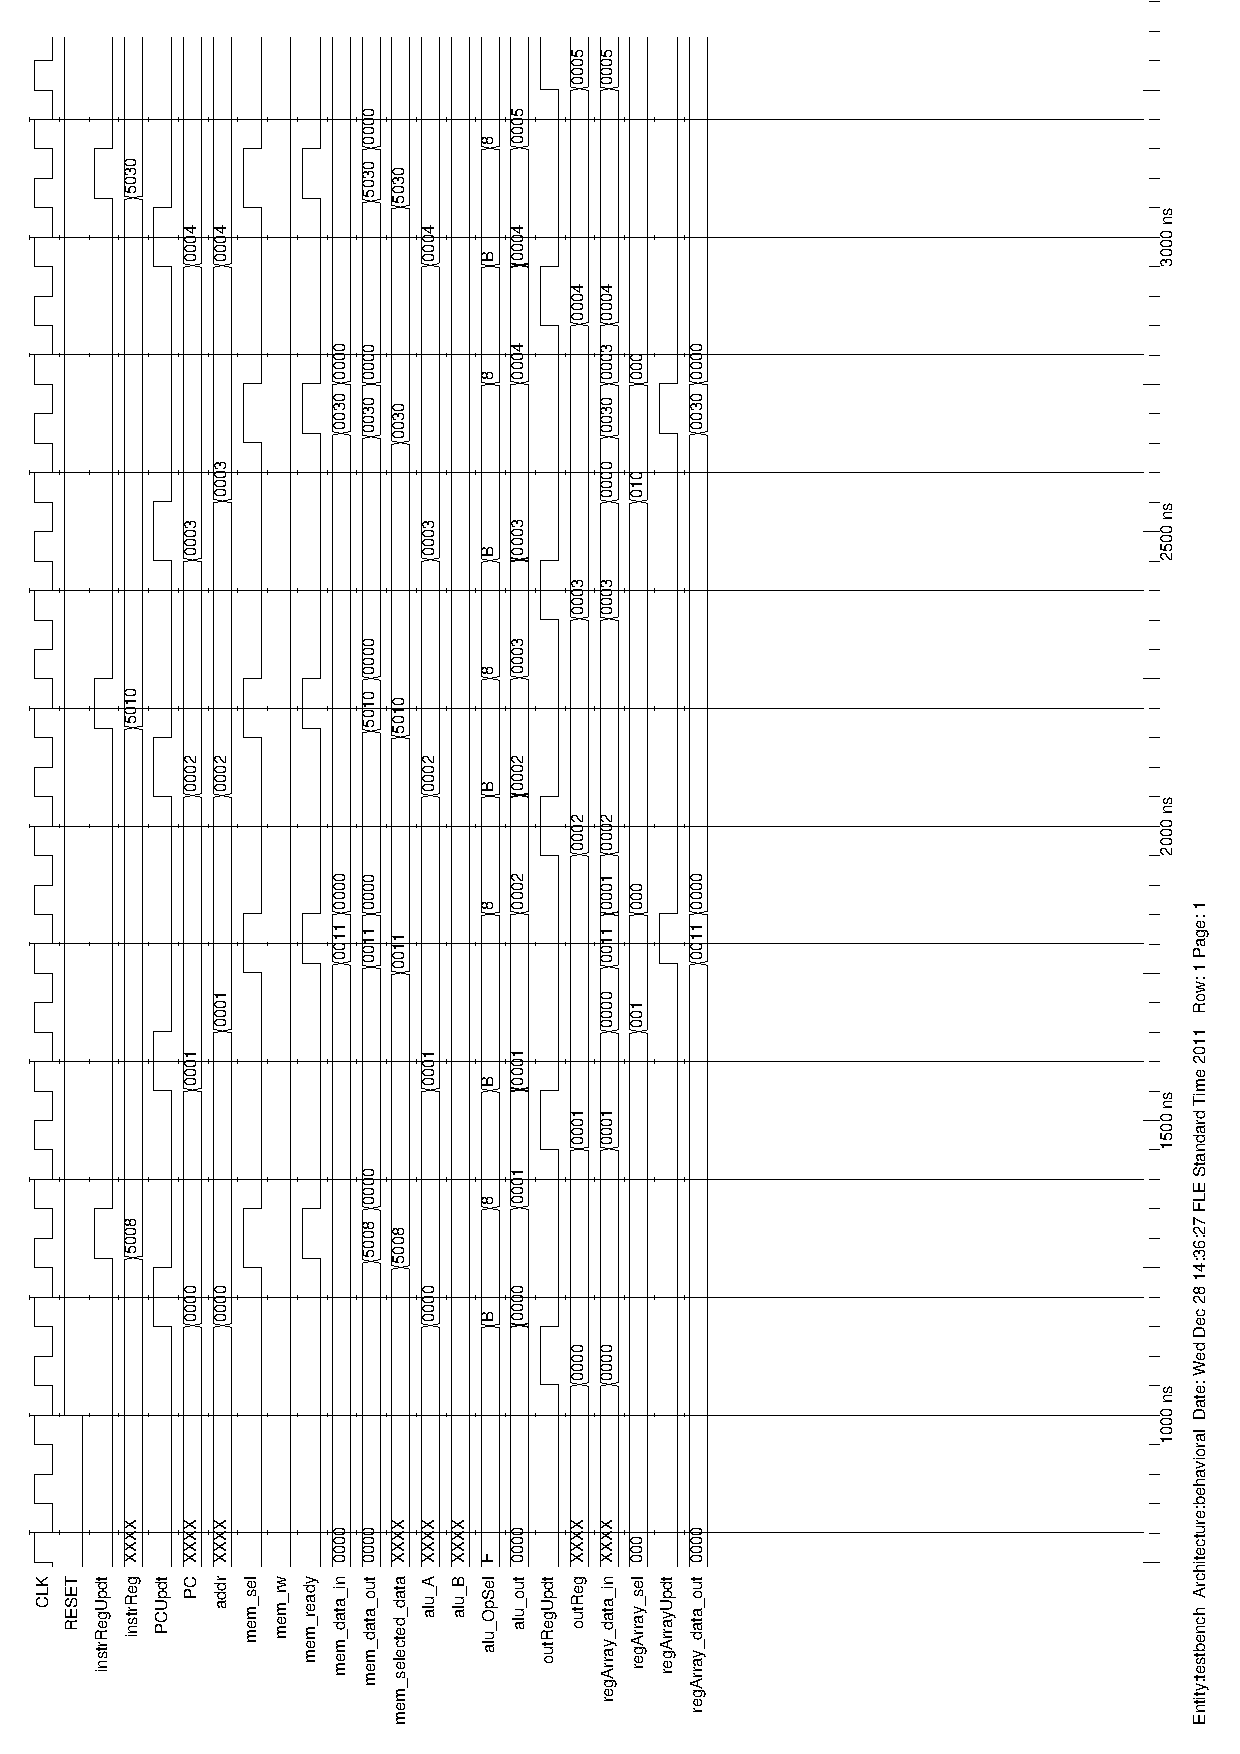
\includegraphics[trim = 0cm 0cm 8cm 0cm,clip,angle=-90,width=\linewidth]{sim0-init}\\
	\caption{Inicializācijas laika diagramma.}
	\label{fig:sim-init}
\end{sidewaysfigure}

\begin{sidewaysfigure}
	\centering
	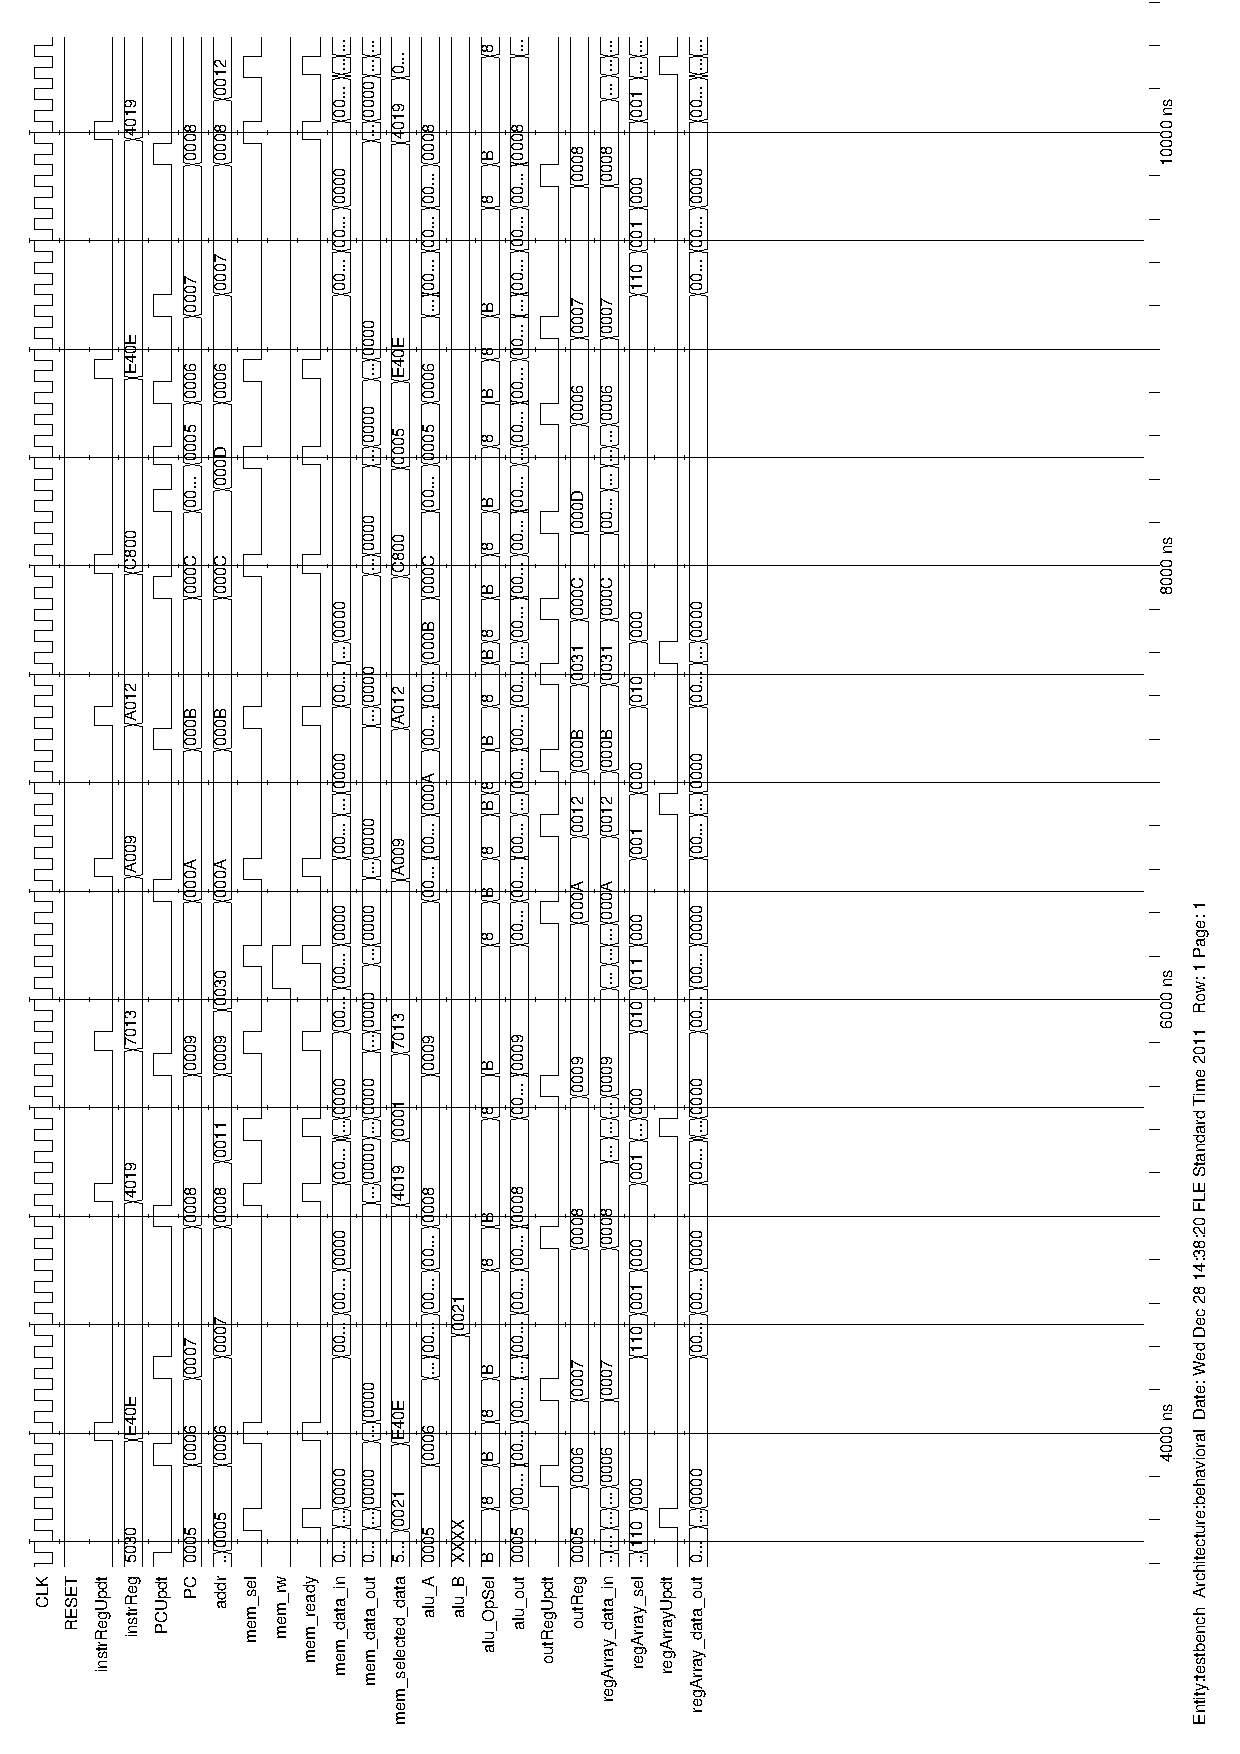
\includegraphics[trim = 0cm 0cm 8cm 0cm,clip,angle=-90,width=\linewidth]{sim0-cycle}\\
	\caption{Programmas cikla izpildes laika diagramma.}
	\label{fig:sim-cycle}
\end{sidewaysfigure}

\begin{sidewaysfigure}
	\centering
	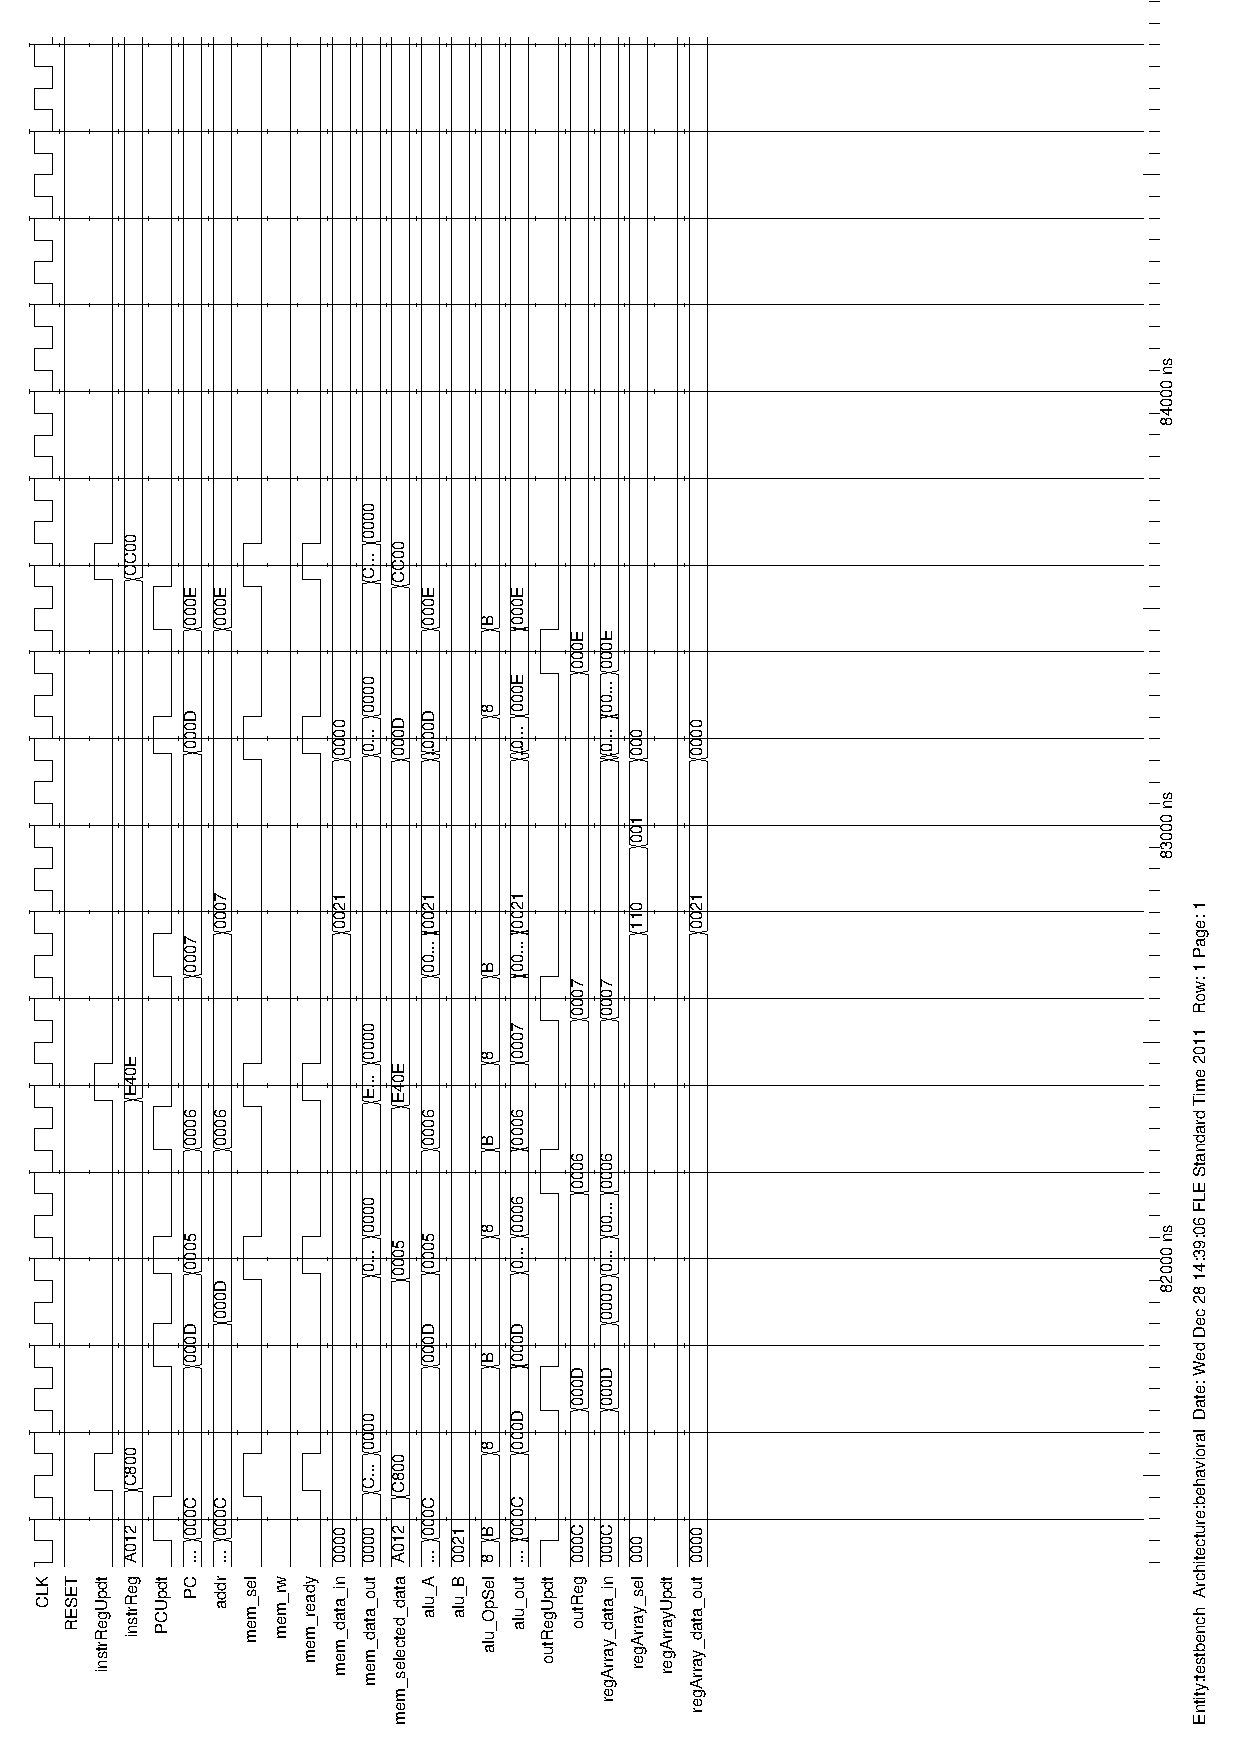
\includegraphics[trim = 0cm 0cm 8cm 0cm,clip,angle=-90,width=\linewidth]{sim0-halt}\\
	\caption{Programmas izpildes beigu laika diagramma.}
	\label{fig:sim-halt}
\end{sidewaysfigure}

\lstinputlisting[float=p,
                 language={JSI},
                 caption={Testa programmas asemblerkods.},
                 basicstyle=\ttfamily\scriptsize,
                 label=kb:copy-program]{code/gen/copy-noaccents.asm}

\clearpage
\section{Paraugimplementācijas asemblerkoda galvene (rev.~03)}
\lstinputlisting[%float=hp,
                 language={JSI},
                 caption={Galvene asemblera programmām (\texttt{JISonFUSIONr3.inc}).},
                 basicstyle=\ttfamily\scriptsize,
                 label=kb:asm-header]{code/JSIonFUSIONr3.inc}

\clearpage
\section{Sāknēšanas programma un simulācijas rezultāti (rev.~03)} \label{appx:boot}
\lstinputlisting[%float=hp,
                 language={JSI},
                 caption={Sāknēšanas programmas asemblerkods.},
                 basicstyle=\ttfamily\scriptsize,
                 label=kb:boot]{code/boot.asm}

\begin{sidewaysfigure}
	\centering
	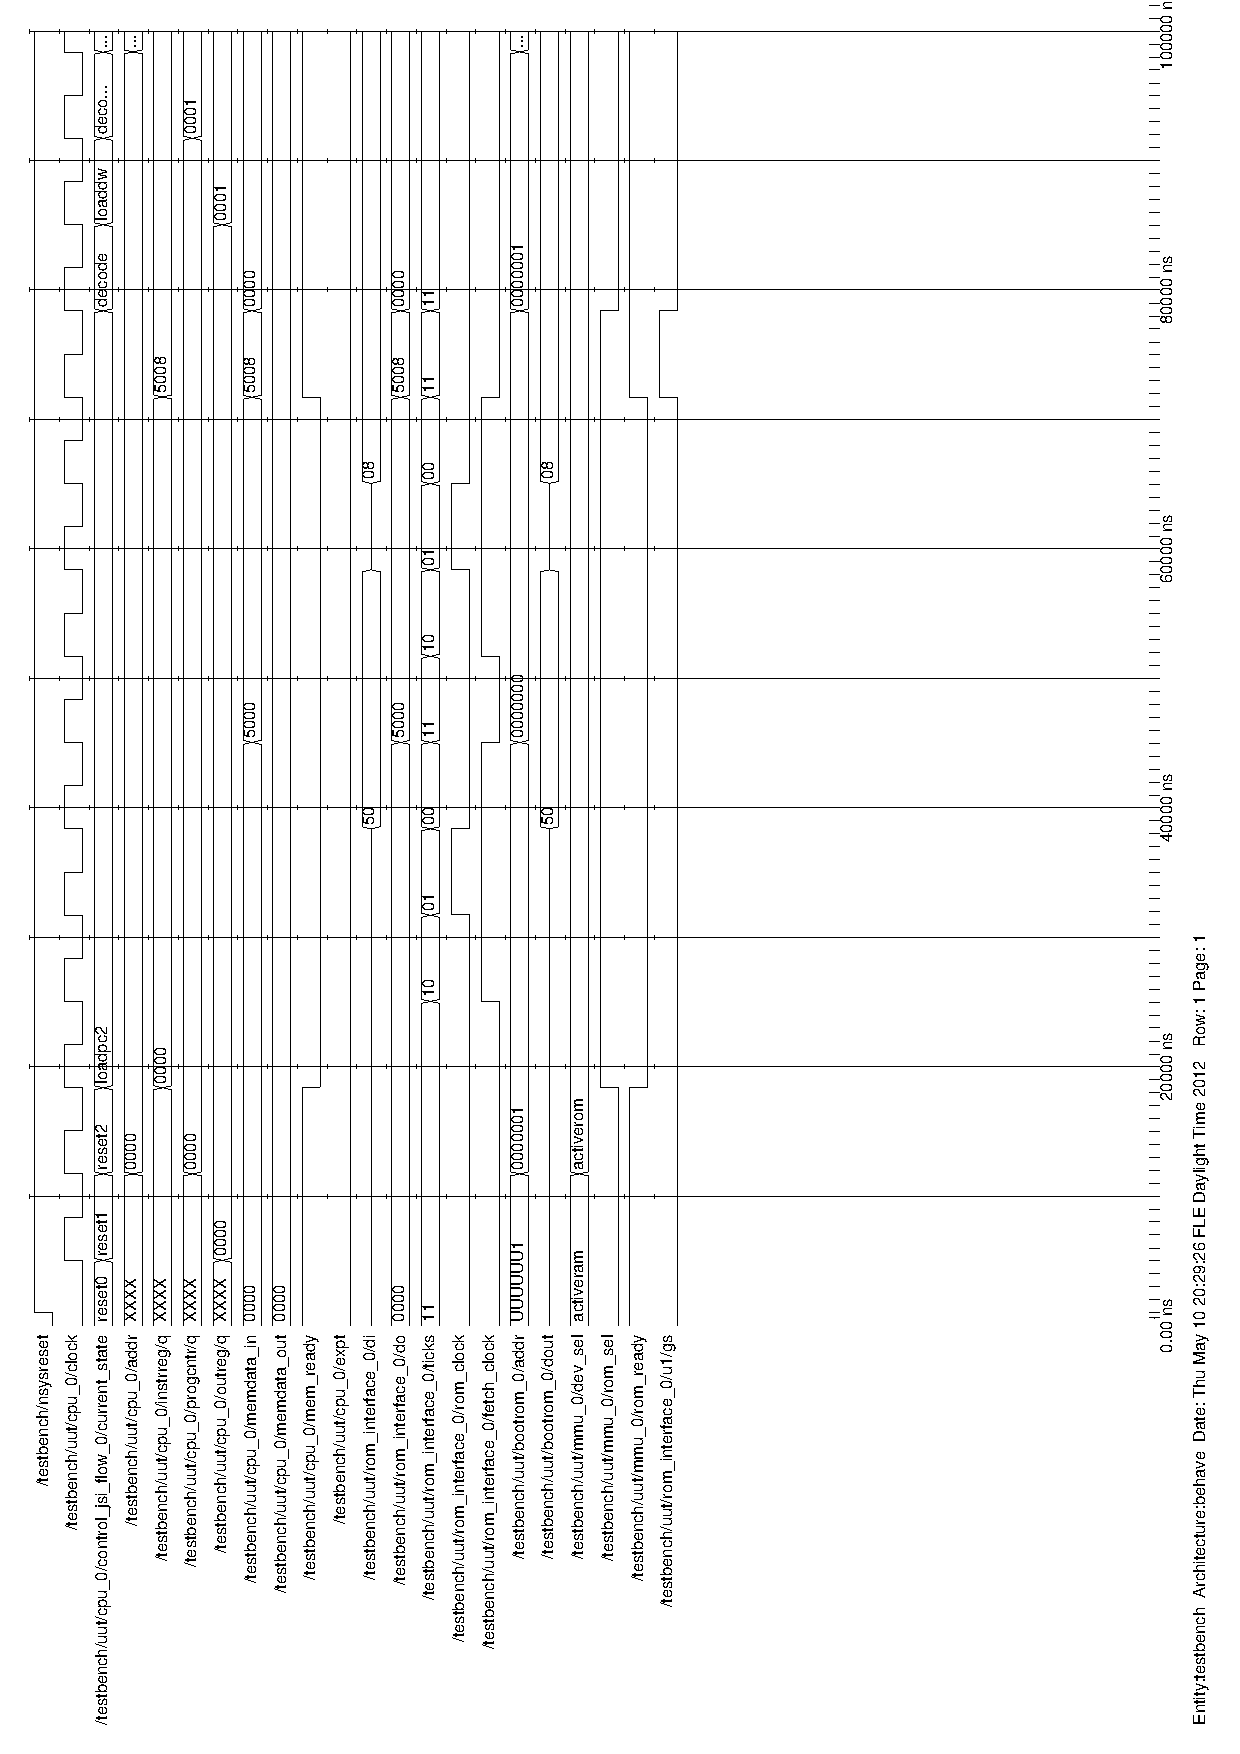
\includegraphics[trim = 0cm 0cm 8.75cm 0cm,clip,angle=-90,width=\linewidth]{sim1_init}\\
	\caption{Mikrokontroliera inicializācijas laika diagramma.}
	\label{fig:sim-boot}
\end{sidewaysfigure}

\begin{sidewaysfigure}
	\centering
	\includegraphics[trim = 0.5cm 0cm 3.25cm 0cm,clip,angle=-90,width=\linewidth]{sim3_tx}\\
	\caption{SPI \termEn{Flash} nolases komandas nosūtīšanas laika diagramma.}
	\label{fig:sim-spi-tx}
\end{sidewaysfigure}

\begin{sidewaysfigure}
	\centering
	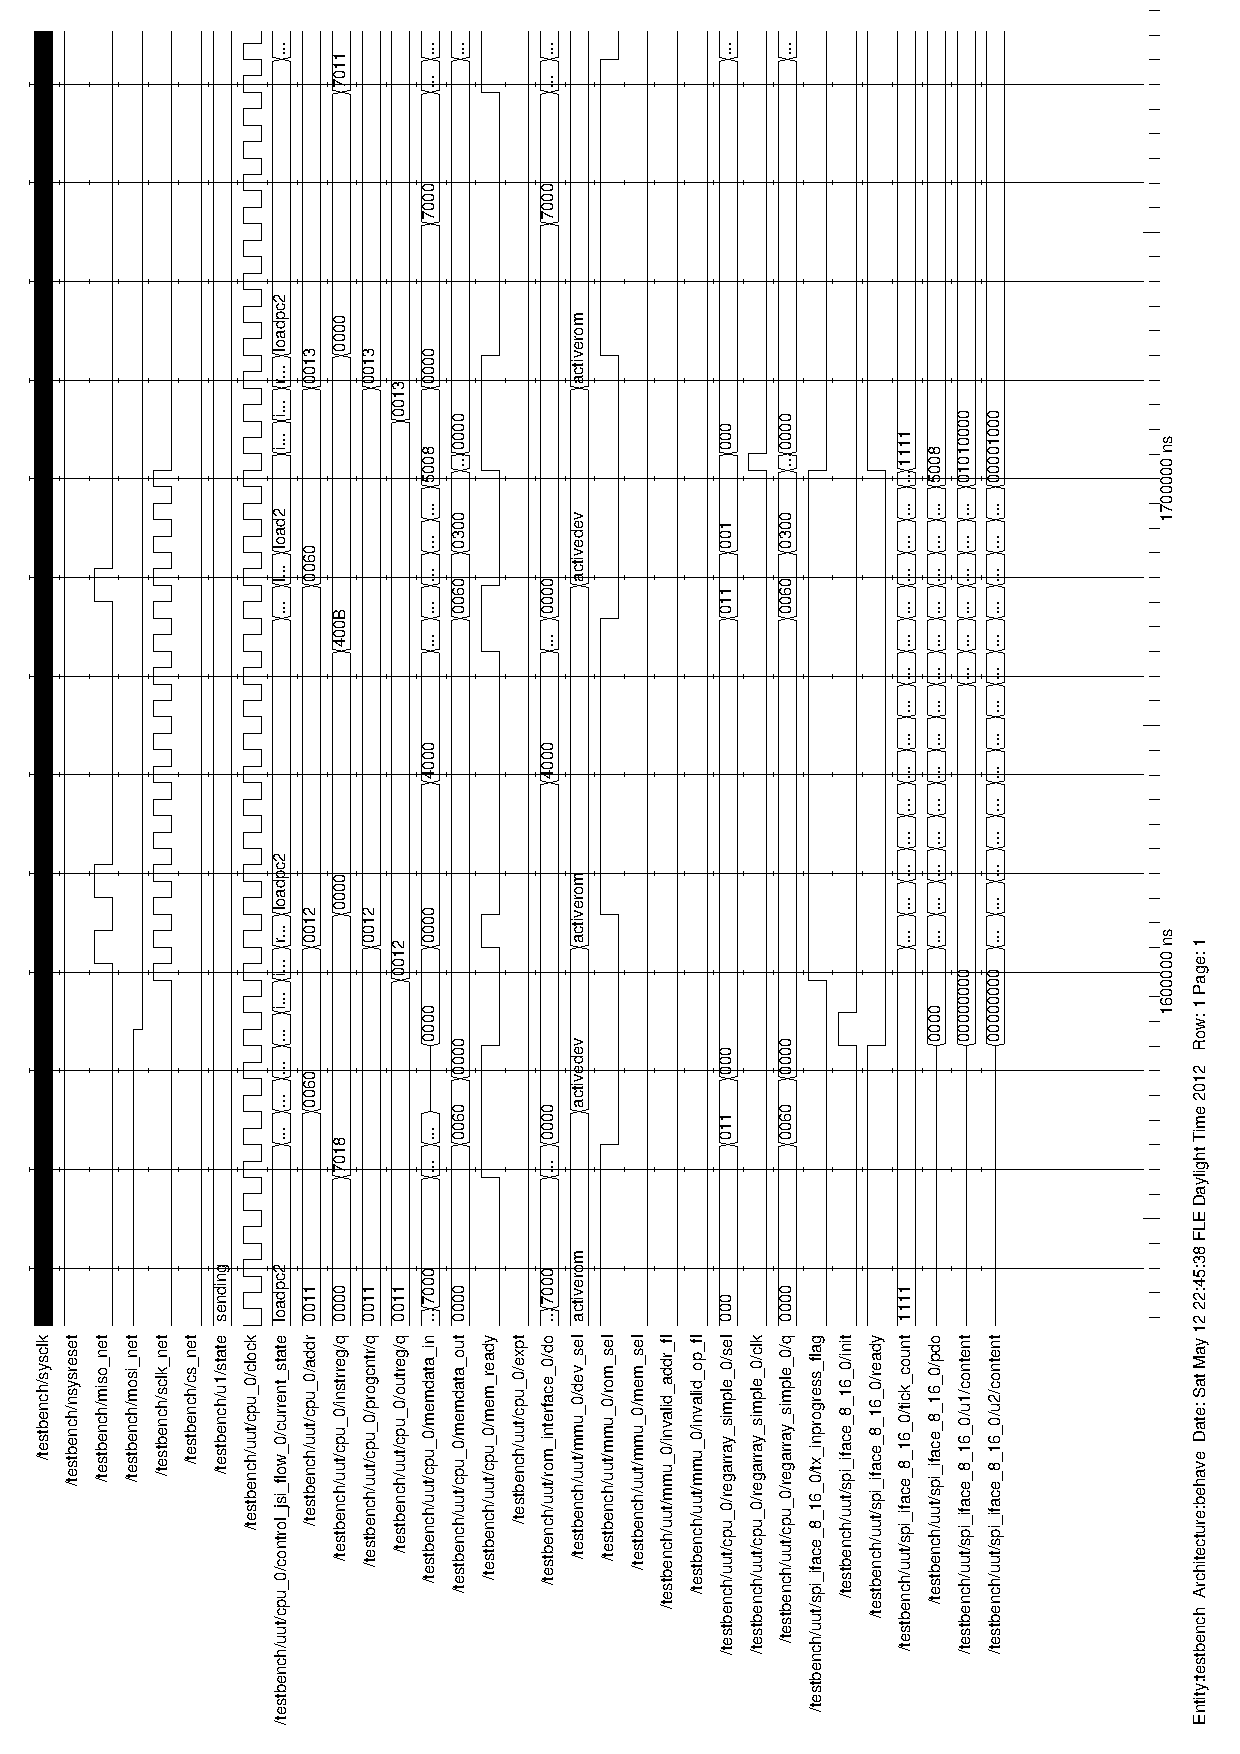
\includegraphics[trim = 0.5cm 0cm 3.25cm 0cm,clip,angle=-90,width=\linewidth]{sim3_rx}\\
	\caption{SPI \termEn{Flash} datu nolases cikla laika diagramma.}
	\label{fig:sim-spi-rx}
\end{sidewaysfigure}

\end{document}
